\documentclass{article}

\title{Project 2 : Graphs and Network Flows}
\author{Aashith Kamath Manjeshwar, Daksha Asrani, Saikrishna Badrinarayanan}
\newcommand{\R}{\mathbf{R}}
%\newcommand{\SS}{\mathsf{S}}
\newcommand{\V}{\mathsf{V}}
\newcommand{\E}{\mathsf{E}}
\newcommand{\neig}{\mathsf{N}}
\newcommand{\rat}{\mathsf{rating}}
\newcommand{\com}{\mathsf{c}}
\newcommand{\predrat}{\mathsf{predicted\_rating}}

\usepackage{amsmath}
\usepackage{graphicx}
\graphicspath{ {plots/} }
\begin{document}
\maketitle

In this project, we create networks from the IMDb movie data and explore their properties. Specifically,
we study the properties of two networks - one based on actors (and actresses) and the other one based on movies. 
The project was coded in the languages R and python.

\paragraph{Problem 1}: \\
First, we download the actor\_movies.txt and actress\_movies.txt files. Each line in the actor\_movies.txt file has an actor
name followed by a list of all the movies that the actor has acted in. The actress file is also represented similarly.
We then merge both the files into one single file. In the process of merging, we remove all actors (or actresses) who have
acted in lesser than 5 movies.\\

\hrule

\paragraph{Problem 2}:\\
From the merged list constructed above, we create a weighted directed graph. The vertex set of the graph 
$\V$ is the set of all actors/actresses in the list. Then, we define a set 
$ S_i = \{m | i \in \V, m \mbox{ is a movie in which i has acted } \}$ for each vertex $i$. After 
creating this set, we define the edges of the graph $\E$ as follows:
$\E = \{(i,j) | i,j \in \V, S_i \cap S_j \neq \emptyset\}$. That is, for every two actors, we define an edge between them
if they have acted in atleast one movie together. We define the weight of this directed edge from vertex $i$ to
vertex $j$ to be $\Big(\frac{|S_i \cap S_j|}{|S_i|}\Big)$ and this completes
the definition of the graph. \\

We next discuss the implementation details of the creation of the graph at a high level.
Before creating the graph, we first create another list to simplify the process. Similar to the merged list created
in the previous question, we create a list in which each line has a movie name followed by the names of all the actors/actresses 
who have acted in that movie. We can create this list by processing the merged list created earlier. Let's call the earlier merged list
as ``actor list'' and the list created now as ``movie list''. We create the graph by representing it in the form of an
edge list. That is, each line of this list has 3 values - the source node, destination node and the weight of that edge. This
completely defines the edges of the graph. The vertices of the graph are the actor/actress names in the actor list.\\
To create the edge list, we iterate through each line in the actor list file. For every actor/actress $i$, we have the list 
of movies he/she has acted in. We iterate through these movies. Now, for each movie, we find that movie in the movie list 
file and look at the list of actors/actresses $L$ who have acted in that movie. For each actor/actress $j$ in this list, such that
$j \neq i$,
We create a directed edge between $i$ and $j$. $S_i$ would be the number of movies $i$ has acted in and this
can be got from the row being processed in the actor list file. Similarly, we can get $S_j$ from the actor list file 
by looking at the row corresponding to $j$. We can compute the edge weight from the above values.
We maintain the edgelist as a set and add the new edge to this set. Since the data structure is represented as a set,
it removes duplicate entries from being added. That is, by the above process, if two actors $i$ and $j$ had acted in multiple movies
together, we would be creating the edge several times. That is prevented from being repeatedly added to the edgelist because
the edgelist is maintained as a set. This completes the process of creating the graph.\\

\hrule

\paragraph{Problem 3}:\\
We run pagerank algorithm on the graph created in the above problem with a damping factor of $0.85$.
Next, we look at the top 10 actors/actresses. That is, the 10 actors/actresses who have the highest average visit
probability. Their names are:
\begin{enumerate}
 \item 
Bess Flowers   
\item 
Sam Harris
\item
Ron Jeremy 
\item
Fred Tatasciore
\item
Harold Miller
\item
Yuri Lowenthal
\item
Eric Roberts
\item
Lee Phelps
\item
Jeffrey Sayre
\item
Franklyn Farnum
\item
Larry Steers
\end{enumerate}
All their pagerank values are in the range from $1*10^{-4}$ to $2*10^{-4}$.
Next, we checked the pairings between them to see how significant they are. That is, to check in how many movies they
have acted together which is indicated in a higher edge weight between that pair. Based on our analysis we make quite a few observations. Firstly, Bess Flowers, Sam Harris, 
Harold Miller, Jeffrey Sayre and Franklyn Farnum are all uncredited extras in tv shows who have each appeared in more than
500 movies/tv shows in the same era (early 1900s). As a result, they have acted together in a lot of movies resulting in high 
edge weights between every pair among them. We enumerate a few weights below for illustration.
\begin{enumerate}
 \item 
 Bess Flowers $\rightarrow$ Sam Harris $0.27$\\
 Sam Harris $\rightarrow$ Bess Flowers $0.19$
 \item
 Bess Flowers $\rightarrow$ Harold Miller $0.25$\\
 Harold Miller $\rightarrow$ Bess Flowers $0.38$
 \item
  Sam Harris $\rightarrow$ Harold Miller $0.29$\\
 Harold Miller $\rightarrow$ Sam Harris $0.28$
 \item
 Harold Miller $\rightarrow$ Jeffrey Sayre $0.23$\\
 Jeffrey Sayre $\rightarrow$ Harold Miller $0.18$
 \item
 Sam Harris $\rightarrow$ Franklyn Farnum $0.18$\\
 Franklyn Farnum $\rightarrow$ Sam Harris $0.19$
 \end{enumerate}
In the above list, each tuple of the form (a b $\rightarrow$ wt) denotes an edge from node a to node b has an edge weight wt.
We notice that for any pair of actors (a,b) the edgeweights in both directions are not equal. This is because the weight 
measures the fraction of a's movies in which b has also acted in. While the total common movies between them will be the same,
the fraction changes because the total number of movies in which each of them has acted is different.\\

Next, we notice that Larry Steers and Lee Phelps are also extras who have acted in a lot of movies. However, they have mainly
acted in movies and not tv shows. They don't have a significant edgeweight with each other or anyone else in the top 10 list
indicating that they haven't acted in too many movies along with any other member of the top 10 list.\\

Yuri Lowenthal and Fred Tatiascore are voice actors which corroborates our evidence that their common movies with any among
the other actors in the top 10 are very few in number. Between them, they seem to have joined forces pretty often as indicated
by the edges below:
\begin{enumerate}
\item
 Yuri Lowenthal $\rightarrow$ Fred Tatiascore $0.23$\\
 Fred Tatiascore $\rightarrow$ Yuri Lowenthal $0.20$
 \end{enumerate}
Jeremy Ron is an adult actor and has no common movies with anyone else on the list.\\

Eric Roberts is a supporting actor who has played a few huge roles in some movies. However, he too has very less in common
with all the others in the list.\\

We hadn't heard about any of the 10 actors in this list before. On delving deeper into their roles, we realized why that was
the case. All of them are not big celebrities or lead actors who have splashed the front pages of newspapers. Rather, they are
mostly people who perform short roles and have acted in a huge number of movies which has influenced their pagerank values being
high. Also, the fact that most of their careers was in the early 1900s makes it very unlikely that we would have known of them.\\

We next list 10 famous actors according to us in no particular order.
\begin{enumerate}
 \item 
 Johnny Depp
 \item
 Morgan Freeman
 \item
 Robert DeNiro
 \item
 Al Pacino
 \item
 Amitabh Bachchan
 \item
 Shahrukh Khan
 \item
 Angelina Jolie
 \item
 Julia Roberts
 \item
 Jessica Alba
 \item
 Meryl Streep
 \end{enumerate}
All their pagerank values are in the range from $2*10^{-5}$ to $5*10^{-5}$ which is significantly lower than the previous list.
This can be attributed to two factors. Firstly, most of them are still in the midst of their acting careers and hence the number
of movies they have acted in is not yet very high while the previous list comprised actors who had already retired and 
acted in a lot of movies. Also, more importantly, the above list consists of lead actors/actresses, who as a result, will not have the time
to act in too many movies at once and hence their total movie count would be fairly low. On the other hand, the previous list
consisted of mostly extras who can act in a huge number of movies every year due to lesser commitments in each movie.
We know that the edgeweights (and hence pagerank values) is proportional to the number of movies each actor has acted
in and hence our top 10 list have a significantly lower pagerank value.\\

The above point also explains why no well known actor/actress shows up in the top pagerank list. That is, well known actors/actresss or 
big celebrities would have acted in far lesser movies than the extras appearing in the list and hence would have a much lesser
pagerank value.\\

Additionally, we observe that the edge weight between any two actors/actresses in the above list is not very high. This 
is because not too many movies have the same set of lead actors. Putting it differently, for each lead actor, with very
high probability, his/her fellow lead actors would not always be the same in all their movies or the fraction of movies
they perform with a fellow lead actor/actress is not usually high. Hence, these edgeweights are quite low.\\
 
\hrule

\paragraph{Problem 4}:\\
Similar to problem 2, we create a weighted graph but in this case, it is undirected. The vertex set of the graph 
$\V$ is the set of all movies. Then, we define a set 
$ S_i = \{a | i \in \V, a \mbox{ is an actor/actress who has acted in movie} i \}$ for each vertex $i$. After 
creating this set, we define the edges of the graph $\E$ as follows:
$\E = \{(i,j) | i,j \in \V, S_i \cap S_j \neq \emptyset\}$. That is, for every two movies, we define an edge between them
if they have atleast one common actor. We define the weight of this directed edge from vertex $i$ to
vertex $j$ to be $\Big(\frac{|S_i \cap S_j|}{|S_i \cup S_j|}\Big)$. We see from this definition weight that the graph is undirected.
This completes the definition of the graph. \\

We next discuss the implementation details of the creation of the graph at a high level.
We create the graph by representing it in the form of an
edge list. That is, each line of this list has 3 values - the source node, destination node and the weight of that edge. This
completely defines the edges of the graph. To create the edge list, we iterate through each line in the movie list 
file. For every movie $i$, we have the list of actors/actresses who have acted in that movie. We iterate through these 
actors/actresses. Now, for each actor/actreses, we look at the actor list file and find the list of movies $L$ that this 
actor/actress has acted in. For each movie $j$ in this list, such that
$j > i$, we create an undirected edge between $i$ and $j$. $S_i$ would be the number of actors/actresses in $i$ and this can
be got from the row being processed in the movie list file. Similarly, we can get $S_j$ from the movie list file 
by looking at the row corresponding to $j$. We can compute the edge weight from the above values.
We maintain the edgelist as a set and add the new edge to this set. Since the data structure is represented as a set,
it removes duplicate entries from being added. That is, by the above process, if two movies $i$ and $j$ had acted in multiple 
movies together, we would be creating the edge several times. That is prevented from being repeatedly added to the edgelist because
the edgelist is maintained as a set. This completes the process of creating the graph.\\

\hrule

\paragraph{Problem 5}:\\
On the above movie network, we first find its giant connected component(GCC) and then the community structure of this 
GCC using the Fast Greedy Newman Algorithm. The GCC of a graph is
a connected component that contains a constant fraction of the entire graph’s
vertices. We find the GCC by first computing the set of clusters in the graph
and then the largest cluster among them. We then delete the vertices that do
not belong to the largest cluster and this gives the GCC.
A network is said to have a community structure if the nodes of the
network can be easily grouped into (potentially overlapping) sets of nodes such
that each set is densely connected internally. The community structure is :
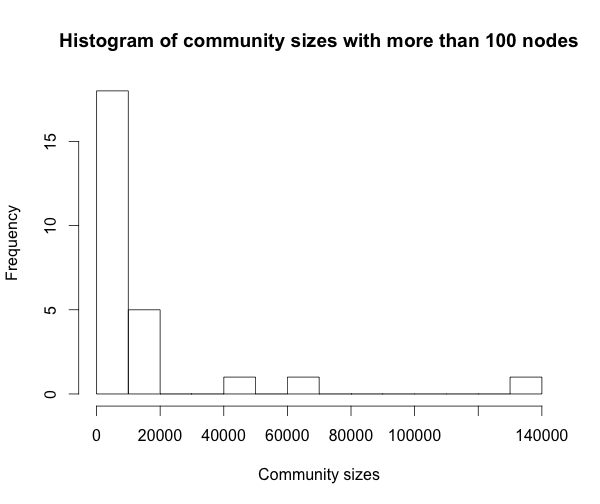
\includegraphics[scale=0.4]{ComSize} \\
The above plot has the community sizes on the x-axis and their corresponding frequencies (i.e the number of communities
with that size) on the y-axis.
The largest community has size $130669$.\\

We know that each movie is associated with a particular genre. We tag each community with a set of genres such that
alteast $20\%$ of the movies in the community have that genre. Most communities had only 1 tag. There were quite a few communities
with 2 or 3 tags and very few with 4 tags. There were no communities with more than 4 tags in them.
For the bigger communities, the tags were not too informative as there are several movies across a varied spectrum
of genres and so we cannot group together the movies in the community to mostly be part of one genre. For example, for the 
biggest community the tag we could assign was ``short'' which means that the movies are of short duration. We know that this 
is not very accurate because we know of several popular full length movies that are part of this community. Some of them
are listed in the subsequent problems. However, though we had movies from several genres, no other genre apart from ``short'' 
had more than $20\%$ movies and this is perhaps the underlying theme behind why the big communities don't have meaningful tags.  
However, the smaller communities did generate meaningful tags. Also, in cases where the community was tagged with more than
1 genre, we observe that the tags were related. For example, one community was tagged with thriller and war. These two tags are
pretty related. Another community was tagged with thriller and mystery. We say they are related because most mystery movies
are thrilling and vice versa and the distinction between them is not easily demarcatable. Another example is a community tagged
with comedy and musical. A classic example is one community that is tagged romance and comedy. We know that several movies
have a good flavour of romance and comedy in equal proportion which in fact has led to the new pseudo-genre name ``romcom''. 

\hrule

\paragraph{Problem 6}:\\
We focus on the following movies for our analysis in this problem :
\begin{enumerate}
 \item 
 Minions (2015)
 \item
 Batman v Superman: Dawn of Justice (2016)
 \item
 Mission: Impossible - Rogue Nation (2015)
\end{enumerate}
For each of these movies, we find their top 5 nearest neighbours. For this, we need a notion of
``distance'' to have a meaningful representation of nearest neighbours. We define the closest neighbour of a movie $i$
to be that movie $j$ such that among all the movies that $i$ has an edge with, the weight of the edge to $j$ is highest.
This implicitly sets the distance between two nodes to be the negative of the edge weight and so the closest neighbours are
the ones who have the largest weight (though the distance becomes negative, that is not a matter of concern as we are only 
interested in the least distance and not it's absolute value).

With this definition of closest neighbours, we list them along with the community to which they belong for each
of the movies we are focussing on.
\begin{itemize}
 \item \textbf{Minions (2015)}\\
 The closest neighbours in the order of closeness are:
 \begin{enumerate}
  \item
  The Lorax (2012) (voice)
  \item
  Inside Out (2015) (voice)
  \item
  Despicable Me2 (2013) (voice)
  \item
  Surf's Up (2015) (voice)
  \item
  WALL-E (2008) (voice) 
 \end{enumerate}
We can observe that all the closest neighbours are voice movies in the last decade preceding the release of Minions.
This is along expected lines because since Minions is a voice movie, a lot of it's cast would comprise of voice actors 
(i.e people whose voice is being played out) and they would probably be part of the cast of several other voice movies in the
last decade. As a result, Minions would have a lot of actors common with these voice movies and hence their edge weight would be 
high leading to closer proximity and them being the nearest neighbours.

\item \textbf{Batman v Superman: Dawn of Justice (2016)}\\
 The closest neighbours in the order of closeness are:
 \begin{enumerate}
 \item
 The Justice League Part One (2017)
  \item
  Eloise (2015) (uncredited)
  \item
 Man of Steel (2013)
 \item
 Home Again (2015)
 \item
 The Double (2011/I) 
 \end{enumerate}
We observe that these results do indeed seem very accurate. This is because the closest neighbour - ``The Justice League Part One (2017)''
is also a batman movie so it shouldn't be surprising at all that several of the cast are common to both the movies!
The movie ``Man of Steel (2013)'' is also very similar to Batman in the sense that it is based on a superhero and the themes
of the movie are quite alike. A quick online search shows that both these movies have the same director and so he could've
involved a lot of people he is comfortable in working with in both these movies leading to a larger edge weight. Another
feature of this set is that all of them are pretty recent movies (and roughly in the same timeline as the Batman movie) which 
increases the probability of having common crew members.

\item \textbf{Mission: Impossible - Rogue Nation (2015)}\\
 The closest neighbours in the order of closeness are:
 \begin{enumerate}
  \item
  Phantom (2015)               
  \item
  The Woman in Black 2: Angel of Death(2014)(uncredited)
  \item
  Fan (2015) 
  \item
  The Mummy Returns (2001)
  \item
  Now You See Me: The Second Act(2016) 
   
 \end{enumerate}
Again, we observe that these results do indeed seem very accurate. 
Firstly, all these movies (along with Mission Impossible) are thriller movies.
Another feature of this set is that all of them are pretty recent movies (except the Mummy Returns).
Both the above indicate that these movies could have a lot of common crew members.



\end{itemize}

We notice that these 3 movies and all their closest neighbours belong to the same community. That is, the entire set of 
18 movies we have listed above belong to the largest community - the one with $130669$ nodes.\\

\hrule

\paragraph{Problem 7}:\\
In this problem, we make use of the ratings file which has a rating associated with most movies in the network.
We notice that for the 3 movies we considered in the previous question there are no ratings given in this file.
This is because these movies are yet to be released. In this problem, we try to predict the ratings of these 3 movies using the method as explained below.\\

For each movie, we look at the 10 closest neighbours of it that have a rating associated with them in the ratings file.
Also, we look at all the movies in the same community of the movie and extract their ratings if available. We take the 
average rating of all thes movies in the same community.
Finally, we take 
an average of this rating and the 10 ratings of the closest neighbours
and predict this to be the rating of the movie under consideration. 
Formally, let $\com(i)$ denote the community to which movie $i$ belongs, 
$\rat(i)$ denote it's rating and $\neig(i)$ denote the set of 10 closest neighbours of movie $i$. The 
predicted rating of movie $m$ is :\\
$$ \predrat(m) = \frac{\Big(\sum\limits_{i \in \neig(m)}\rat(i) + 
  \dfrac{\sum\limits_{\substack{i \in \V \\ \com(i) = \com(m)}}\rat(i)}
  {\sum\limits_{\substack{i \in \V \\ \com(i) = \com(m)}}1}
  \Big)}
  {        \Big( |\neig(m)|+ 1 \Big)      
  }
  $$.
By the above function, the predicted ratings for the 3 movies are:\\
\begin{enumerate}
 \item 
 Minions (2015) - 7.83
 \item
 Batman v Superman: Dawn of Justice (2016) - 7.48
 \item
 Mission: Impossible - Rogue Nation (2015) - 7.44
 
\end{enumerate}

The above predictions do seem very plausible. We claim this because, personally we expect all these 3 movies
to get a high rating considering their cast, genre and the past history of the movies in that series or the books on which
they were based. Our predictions seem to give them a high enough rating to indicate they would be well received by people 
but not too high to unequivocally claim it to be a huge success.\\

\hrule

\paragraph{Problem 8}:\\
Similar to the previous problem, the goal here also is to predict the ratings for those three movies under consideration.
However, unlike in the previous case where we derived a function for predicting its rating, we will use a learning 
approach here. We will build a regression model using all the other movies in the network as the training data and these three
movies as the testing data. The features we considered are the following:
\begin{enumerate}
 \item 
 Top 5 pageranks of the actors/actresses in the movie.
 \item
 A boolean value that is 1 if the director of the movie belongs to the top 100 directors or not. The top 100 directors
 are defined to be the ones who directed the movies that appeared in the top 100 of the ``IMDb top 250'' list.
 \item
 For each actor, we define a rating value that is equal to the average of all the movies he has acted in. After generating this,
 we include the rating of the top 3 actors of the movie as a feature. The idea behind this feature is that a movie gets its
 high rating partly because of the fan base of the lead actors. We would expect a very popular lead actor to have high ratings
 for all his movies and so we incorporated this into the actor by averaging all his movies' ratings as his rating. Now, we expect
 the top 3 actor ratings of a movie to ideally denote the ratings of it's top 3 lead actors and hence if this value is high, its
 very likely that the movie would be favourably received and get a good rating. 
 \item
 Ratings of the top 10 neighbours of the movie. This was one of the parameters considered
 in the previous question when we derived a function for prediction.
 \item
 Average rating of all the movies in the same community as the movie under consideration.
\end{enumerate}
Based on these features, we built the regression model. The $R^2$ value is $0.1392$. We know that closer the value is to 1,
better the fit. We also know that in regression, when we add more features, the $R^2$ value does increase, but not by a huge amount.\\

Now, we predict the ratings for these 3 movies and it turns out as follows:
\begin{enumerate}
 \item 
 Minions (2015) - 6.32
 \item
 Batman v Superman: Dawn of Justice (2016) - 6.84
 \item
 Mission: Impossible - Rogue Nation (2015) - 6.47
 
\end{enumerate}
As in the previous question, the above predictions do seem very plausible. The reasoning for this claim is same as before
and we write it here for completeness.
We claim this because, personally we expect all these 3 movies
to get a high rating considering their cast, genre and the past history of the movies in that series or the books on which
they were based. Our predictions seem to give them a high enough rating to indicate they would be well received by people 
but not too high to unequivocally claim it to be a huge success.
However, the fact that our fit was not very accurate as evidenced by the $R^2$ value explains why our predicted ratings
in this problem are lesser than in the previous one. One issue could be that our pagerank values are not ideal. In the sense that,
as we saw in problem 3, the actors with the highest pagerank values are not the most popular ones or the ones with best
acting capabilities but the ones who were extras and acted in a lot of movies. Ideally, we would like the most famous
or the lead actors to have the highest pagerank values and hence this could be affecting our prediction.
Also, the issue with the actor rating feature is that the top 3 actor ratings
 of a movie need not correspond to the top 3 lead actors of that movie. That is, it could have been for some random uncredited 
 actor who happened to have a high one because of acting in only top rated movies 
 or this turned out to be higher than the lead actors because they were not very good.
 In such a case, we perceive the movie to have a high rating but in reality, it's lead actors have a bad rating. The main underlying 
 issue is that we don't have a way to isolate the lead actors of a movie with the dataset at hand and this is affecting the 
 feature set under consideration.
Also, the rating for a movie may depend on several other parameters 
like how the movie was received by the audience even if the cast was filled with exceptional or popular actors. Also, other
parameters like whether the movie release coincided with that of another very popular movie may also affect its rating
as people might rate it relative to the other movie which could turn out to be good or bad. Hence, the predicted rating here
may not be the most accurate.

\end{document}
